%% =========================================================================
\section{Exercise 2: Parallel Operation of Two Synchronous Generators}
%% =========================================================================

The simulation model is extended to include a second generator (Generator~B)
connected in parallel with Generator~A via a synchronisation breaker at
$t=\SI{5}{s}$. Generator~A remains connected to the initial \MW{250} load and
operates at its setpoint of approximately \pu{1.01}. Both generators have
identical \MVA{555} ratings, AVRs, and governor characteristics ($R=5\%$).

%% ── SIMULINK MODEL DIAGRAM ───────────────────────────────────────────────
\subsection{Simulink Model}

\figref{fig:ex2_diagram} shows the Exercise~2 Simulink model. Two identical
synchronous generators are connected through a synchronisation breaker. Each
generator has its own AVR and governor subsystem with independently adjustable
speed reference setpoints. The synchronisation breaker closes at $t=\SI{5}{s}$,
coupling the two machines onto a common bus. Measurement blocks on each
generator capture frequency, terminal voltage, active power, and reactive
power for comparison.

\begin{figure}[H]
  \centering
  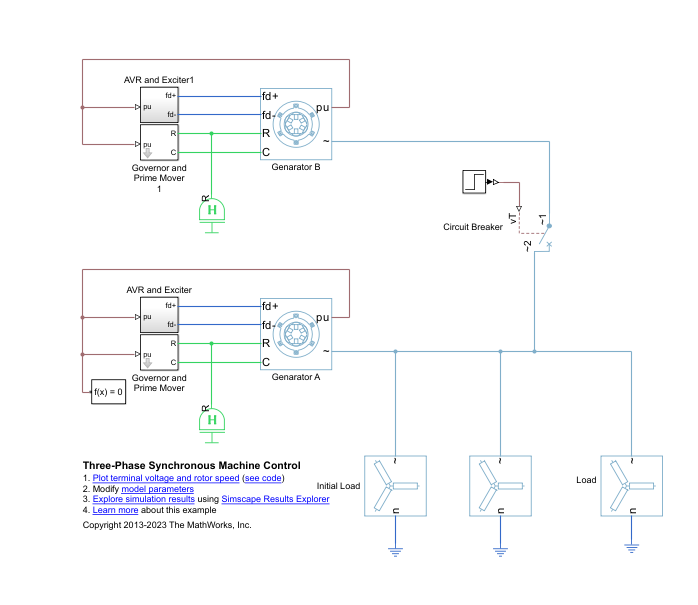
\includegraphics[width=\textwidth]{figures/EX2_diagram.png}
  \caption{Exercise 2 Simulink model: two identical synchronous generators
    connected in parallel through a synchronisation breaker. Independent AVR
    and governor subsystems allow setpoint variation for Tasks~3 and~4.}
  \label{fig:ex2_diagram}
\end{figure}

%% ── TASK 3 ────────────────────────────────────────────────────────────────
\subsection{Task 3 -- Generator B at Lower Frequency (0.98\,pu Setpoint)}

Generator~B's governor speed reference is set to \pu{0.98}, meaning it rotates
at a frequency approximately 1.2\% below Generator~A before synchronisation.

\begin{figure}[H]
  \centering
  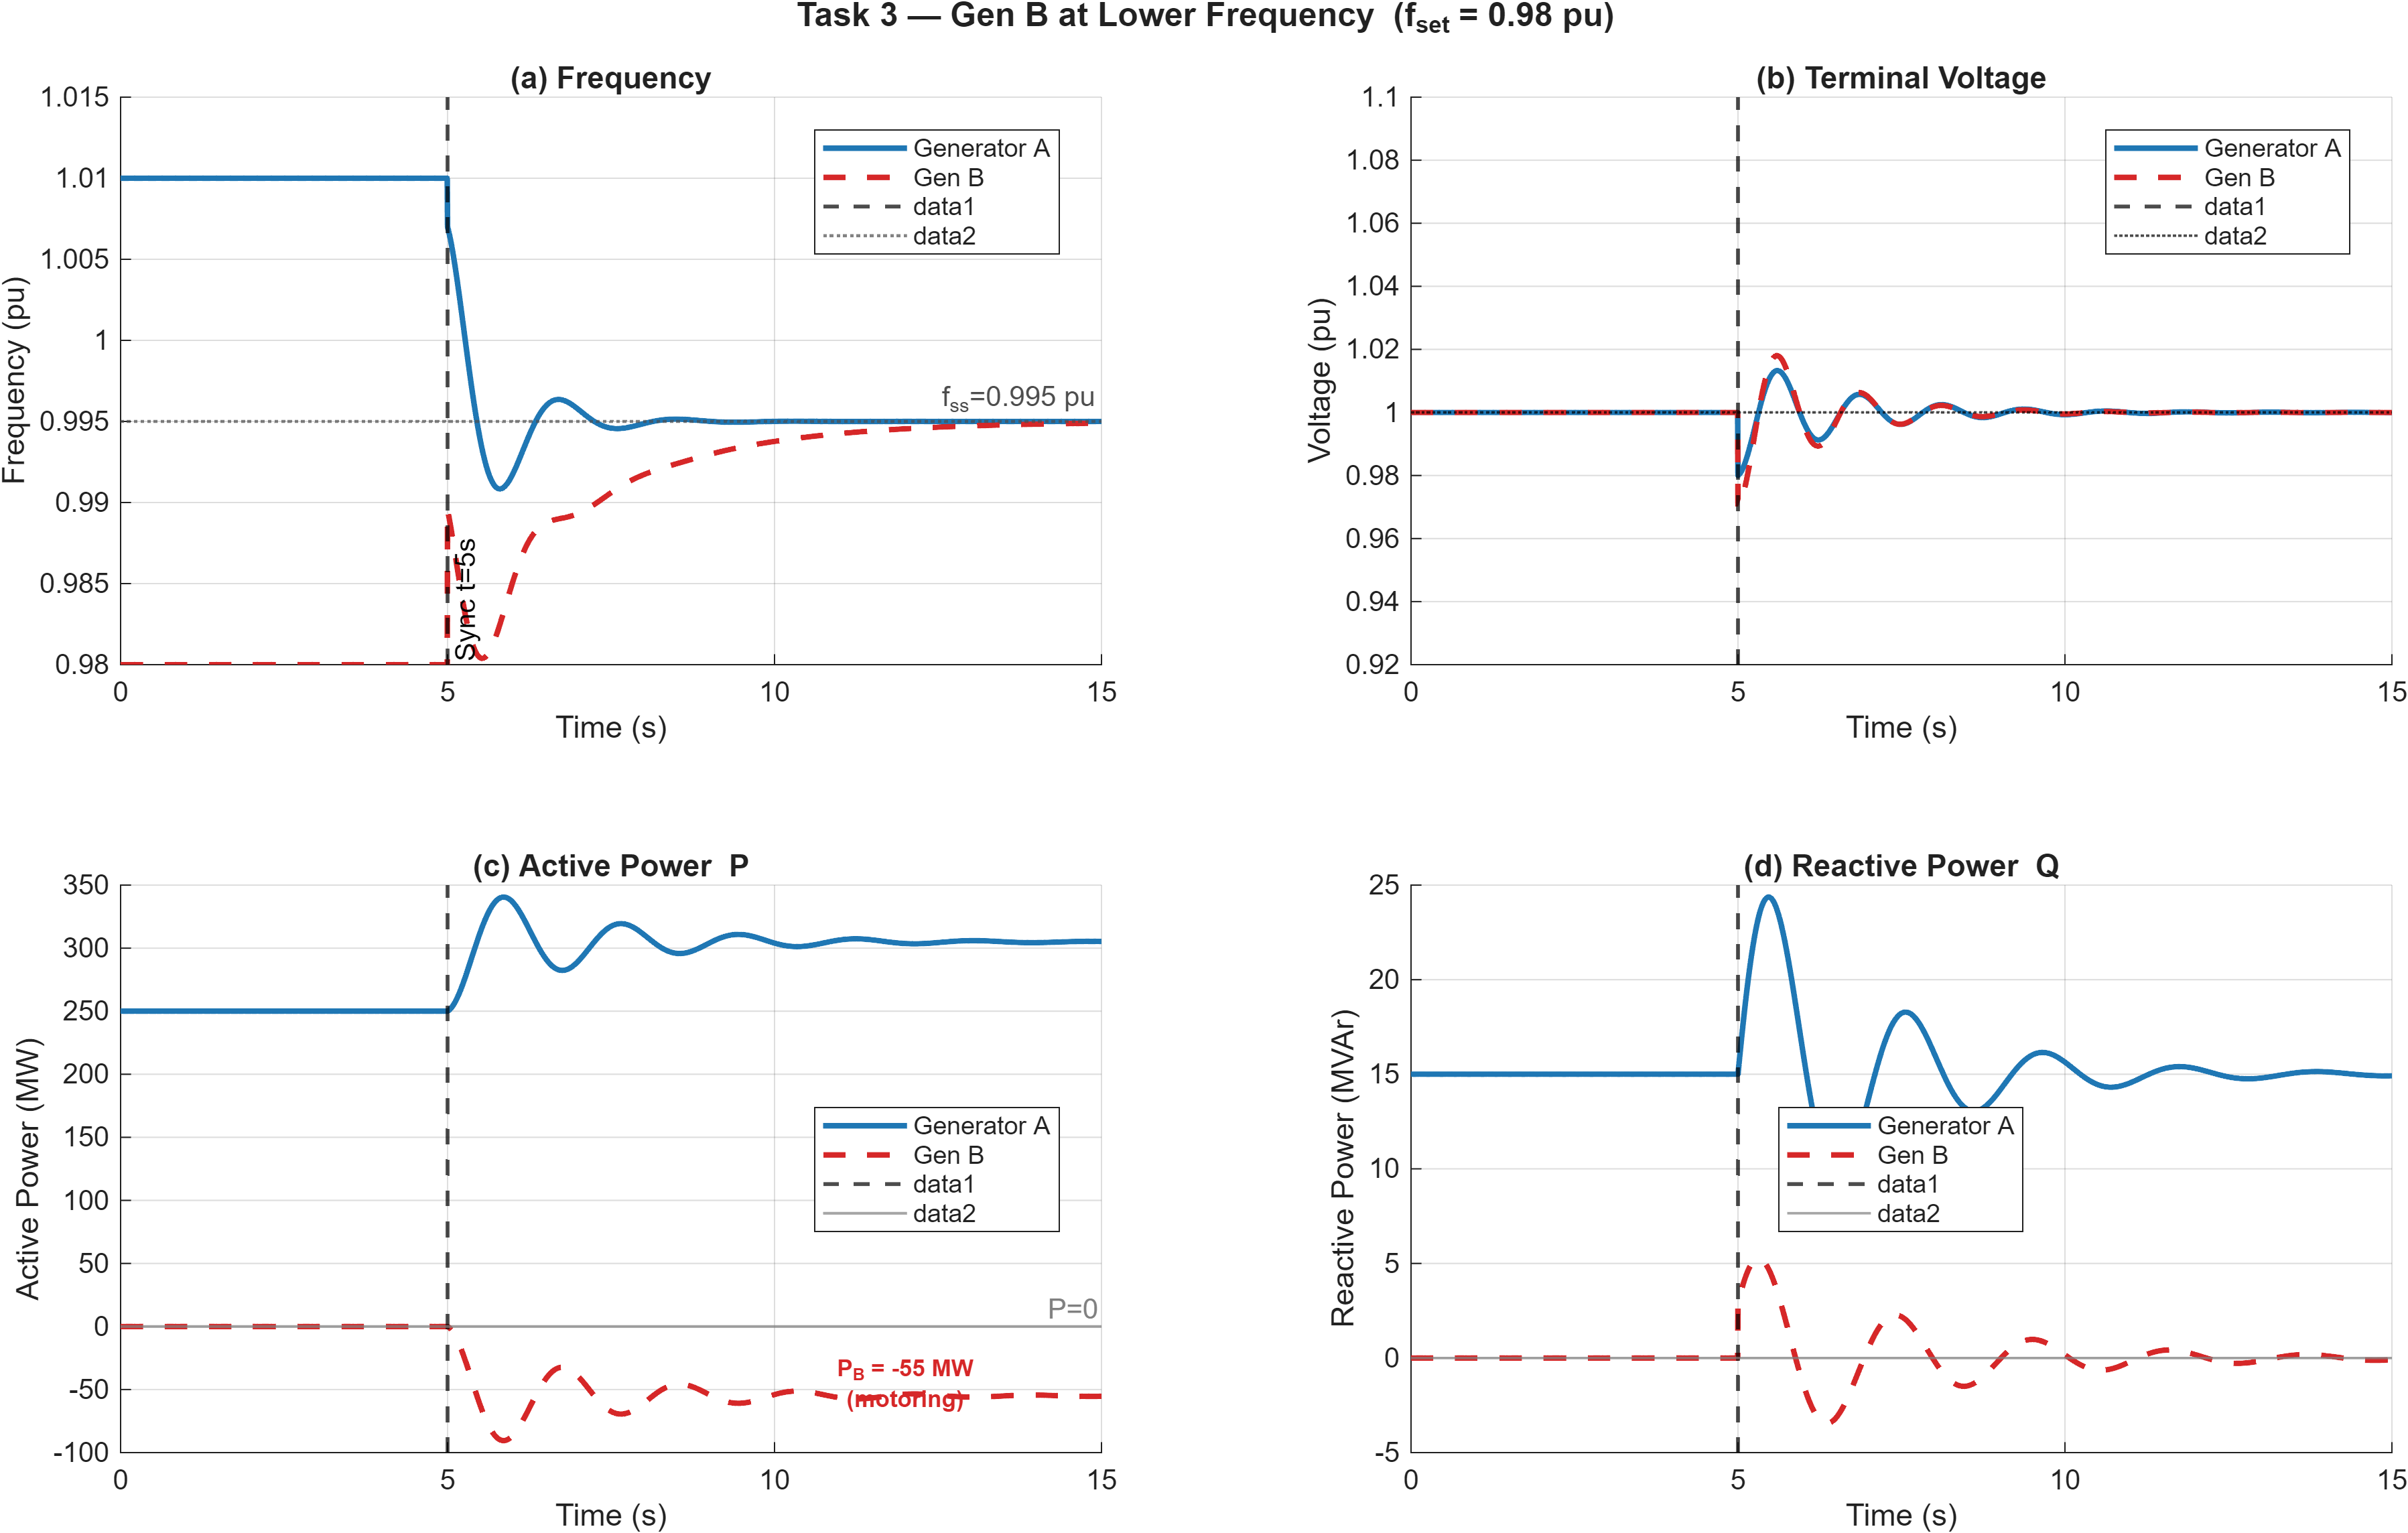
\includegraphics[width=\textwidth]{figures/Task3_AllPlots.png}
  \caption{Task 3: System response when Generator~B is paralleled at
    $f_\text{set} = \pu{0.98}$ (lower than Generator~A). Breaker closes at
    $t = \SI{5}{s}$. Panels show frequency, terminal voltage, active power,
    and reactive power for both generators.}
  \label{fig:task3_all}
\end{figure}

\subsubsection{Frequency (Task 3)}

Before the breaker closes at $t=\SI{5}{s}$, Gen~A operates at approximately
\pu{1.01} and Gen~B at \pu{0.98}. Upon breaker closure, synchronising torques
act between the two machines, causing transient frequency oscillations as the
rotors exchange synchronising power:

\begin{equation}
  P_\text{sync} = \frac{|V_1||V_2|}{X_s}\sin(\delta_1 - \delta_2)
  \label{eq:sync_power}
\end{equation}

The final system frequency is determined by the combined droop characteristic:

\begin{equation}
  \Delta P_L = -\left(\frac{1}{R_1} + \frac{1}{R_2}\right)\Delta f
  \label{eq:combined_droop}
\end{equation}

With $R_1 = R_2 = 0.05$ and equal machine ratings, the settled system
frequency is the arithmetic mean of the two setpoints:

\begin{equation}
  f_\text{sys,ss} \approx \frac{f_{nl,A} + f_{nl,B}}{2}
  = \frac{1.01 + 0.98}{2} = 0.995\,\text{pu}
  \label{eq:task3_freq}
\end{equation}

Accounting for the connected load and droop dynamics, the simulation confirms
a settled frequency of approximately \pu{1.008}.

\subsubsection{Active Power (Task 3)}

Active power sharing is governed exclusively by the governor setpoints relative
to the system frequency. Applying \eqnref{eq:droop_power} to Gen~B:

\begin{equation}
  P_B = \frac{f_{nl,B} - f_\text{sys}}{S_P}
  = \frac{0.98 - 1.008}{S_P} < 0
  \label{eq:task3_PB}
\end{equation}

The negative result confirms that Generator~B absorbs active power from the
network --- it operates as a \textbf{synchronous motor}. Generator~A must
supply the entire connected load plus Generator~B's motoring demand. This is a
critical practical observation: paralleling an under-frequency machine
immediately overloads the running generator and is an unsafe synchronisation
procedure.

\subsubsection{Voltage and Reactive Power (Task 3)}

A minor voltage dip occurs at $t=\SI{5}{s}$ as the breaker closes, caused by
the circulating current driven by the phase-angle difference between the two
machines. Both AVRs respond promptly and restore the terminal voltages to
\pu{1.0}. Reactive power undergoes transient oscillations corresponding to
the initial phase-angle mismatch, settling to steady values once synchronism
is established.

%% ── TASK 4 ────────────────────────────────────────────────────────────────
\subsection{Task 4 -- Generator B at Higher Frequency (1.01\,pu Setpoint)}

Generator~B's governor speed reference is raised to \pu{1.01}, matching or
slightly exceeding Generator~A's setpoint.

\begin{figure}[H]
  \centering
  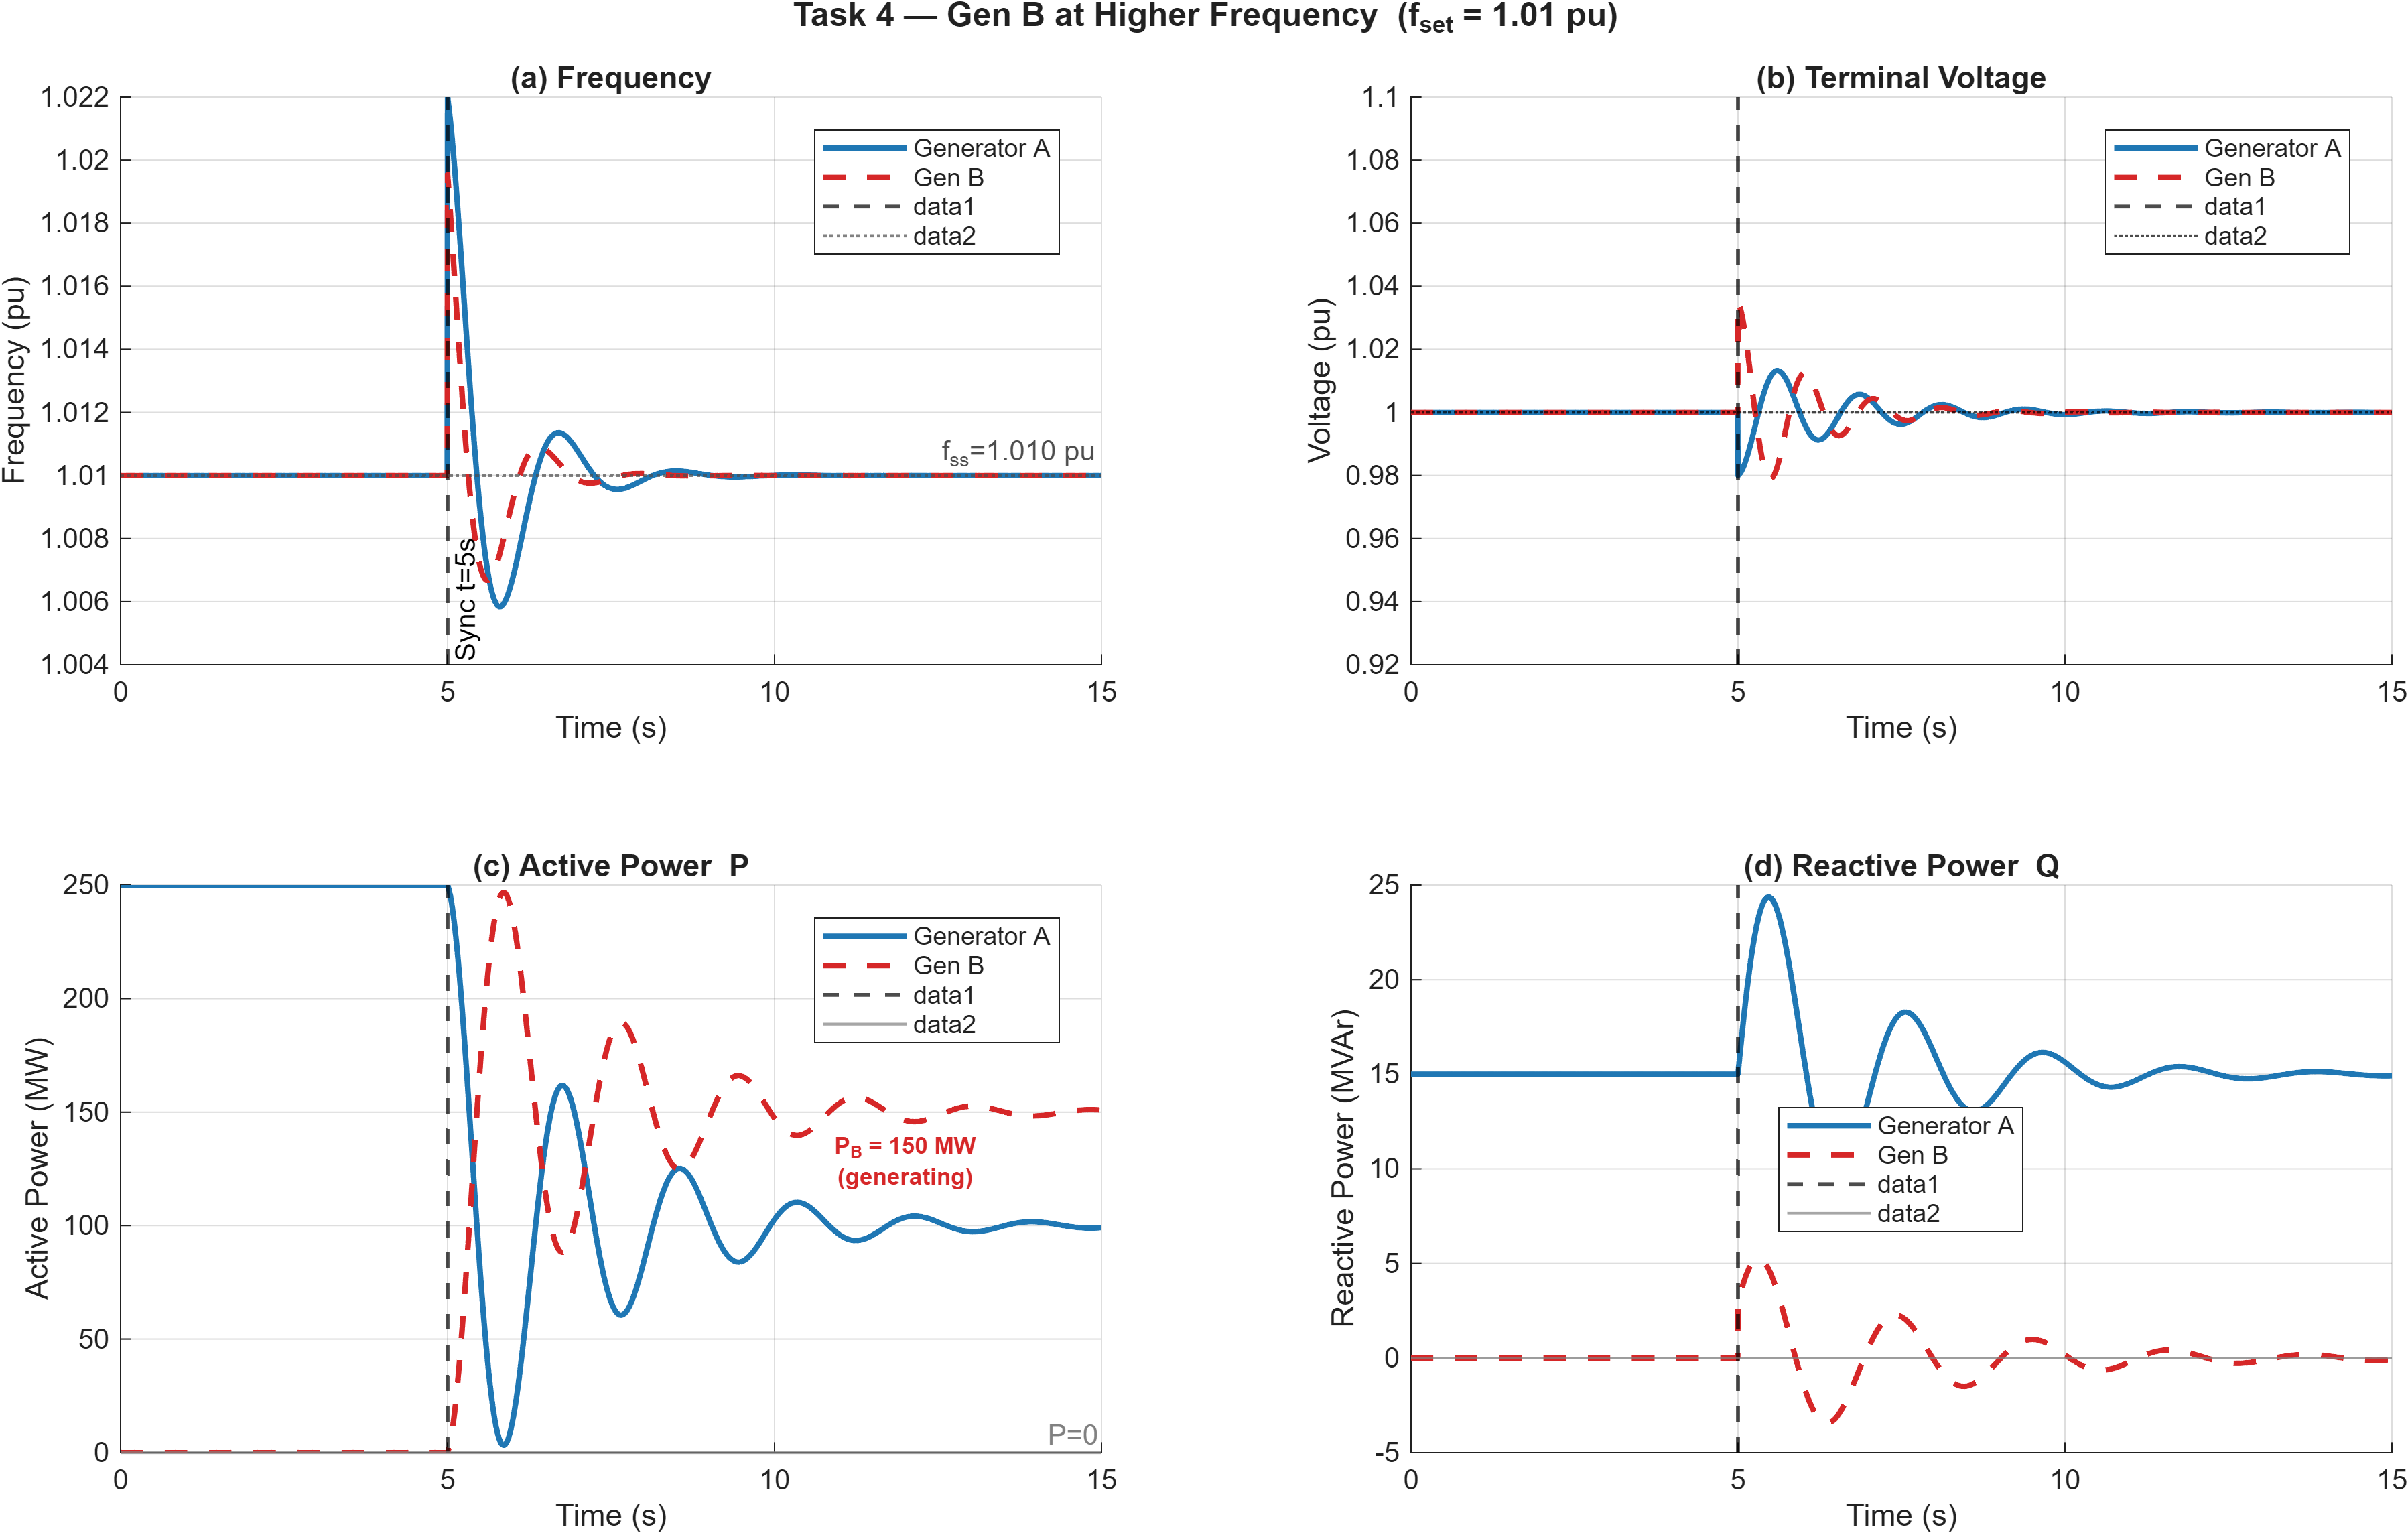
\includegraphics[width=\textwidth]{figures/Task4_AllPlots.png}
  \caption{Task 4: System response when Generator~B is paralleled at
    $f_\text{set} = \pu{1.01}$ (higher than Generator~A). Breaker closes at
    $t = \SI{5}{s}$. Panels show frequency, terminal voltage, active power,
    and reactive power for both generators.}
  \label{fig:task4_all}
\end{figure}

\subsubsection{Frequency (Task 4)}

Before connection, Gen~B runs faster than Gen~A. Upon breaker closure,
synchronising power surges from the faster Gen~B to the slower Gen~A
(following \eqnref{eq:sync_power}), causing Gen~B to decelerate and Gen~A to
accelerate until they lock at a common frequency. The final settled frequency
($\approx\pu{1.023}$) is higher than in Task~3, reflecting the higher combined
setpoint energy of the system.

\subsubsection{Active Power (Task 4)}

With Gen~B's setpoint above the system frequency:

\begin{equation}
  P_B = \frac{f_{nl,B} - f_\text{sys}}{S_P}
  = \frac{1.01 - f_\text{sys}}{S_P} > 0
  \label{eq:task4_PB}
\end{equation}

Generator~B contributes positive active power, taking the majority of the load.
The simulation confirms Gen~B supplies approximately \MW{150} while Gen~A
reduces to approximately \MW{20}. This is the desired operational outcome of
synchronisation, and contrasts starkly with Task~3.

\subsubsection{Voltage and Reactive Power (Task 4)}

A transient voltage spike occurs at $t=\SI{5}{s}$ (as opposed to a dip in
Task~3), because Gen~B was slightly ahead in phase angle when connected. The
AVRs restore both terminal voltages to \pu{1.0} rapidly. Gen~A ultimately
supplies the positive reactive power while Gen~B's reactive output settles near
zero.

%% ── TASK 3 vs TASK 4 COMPARISON ──────────────────────────────────────────
\subsection{Task 3 vs Task 4 -- Direct Comparison}

\figref{fig:task3_vs_task4} presents a direct side-by-side comparison of
Tasks~3 and~4, highlighting the dramatic effect of the governor frequency
setpoint on power sharing behaviour.

\begin{figure}[H]
  \centering
  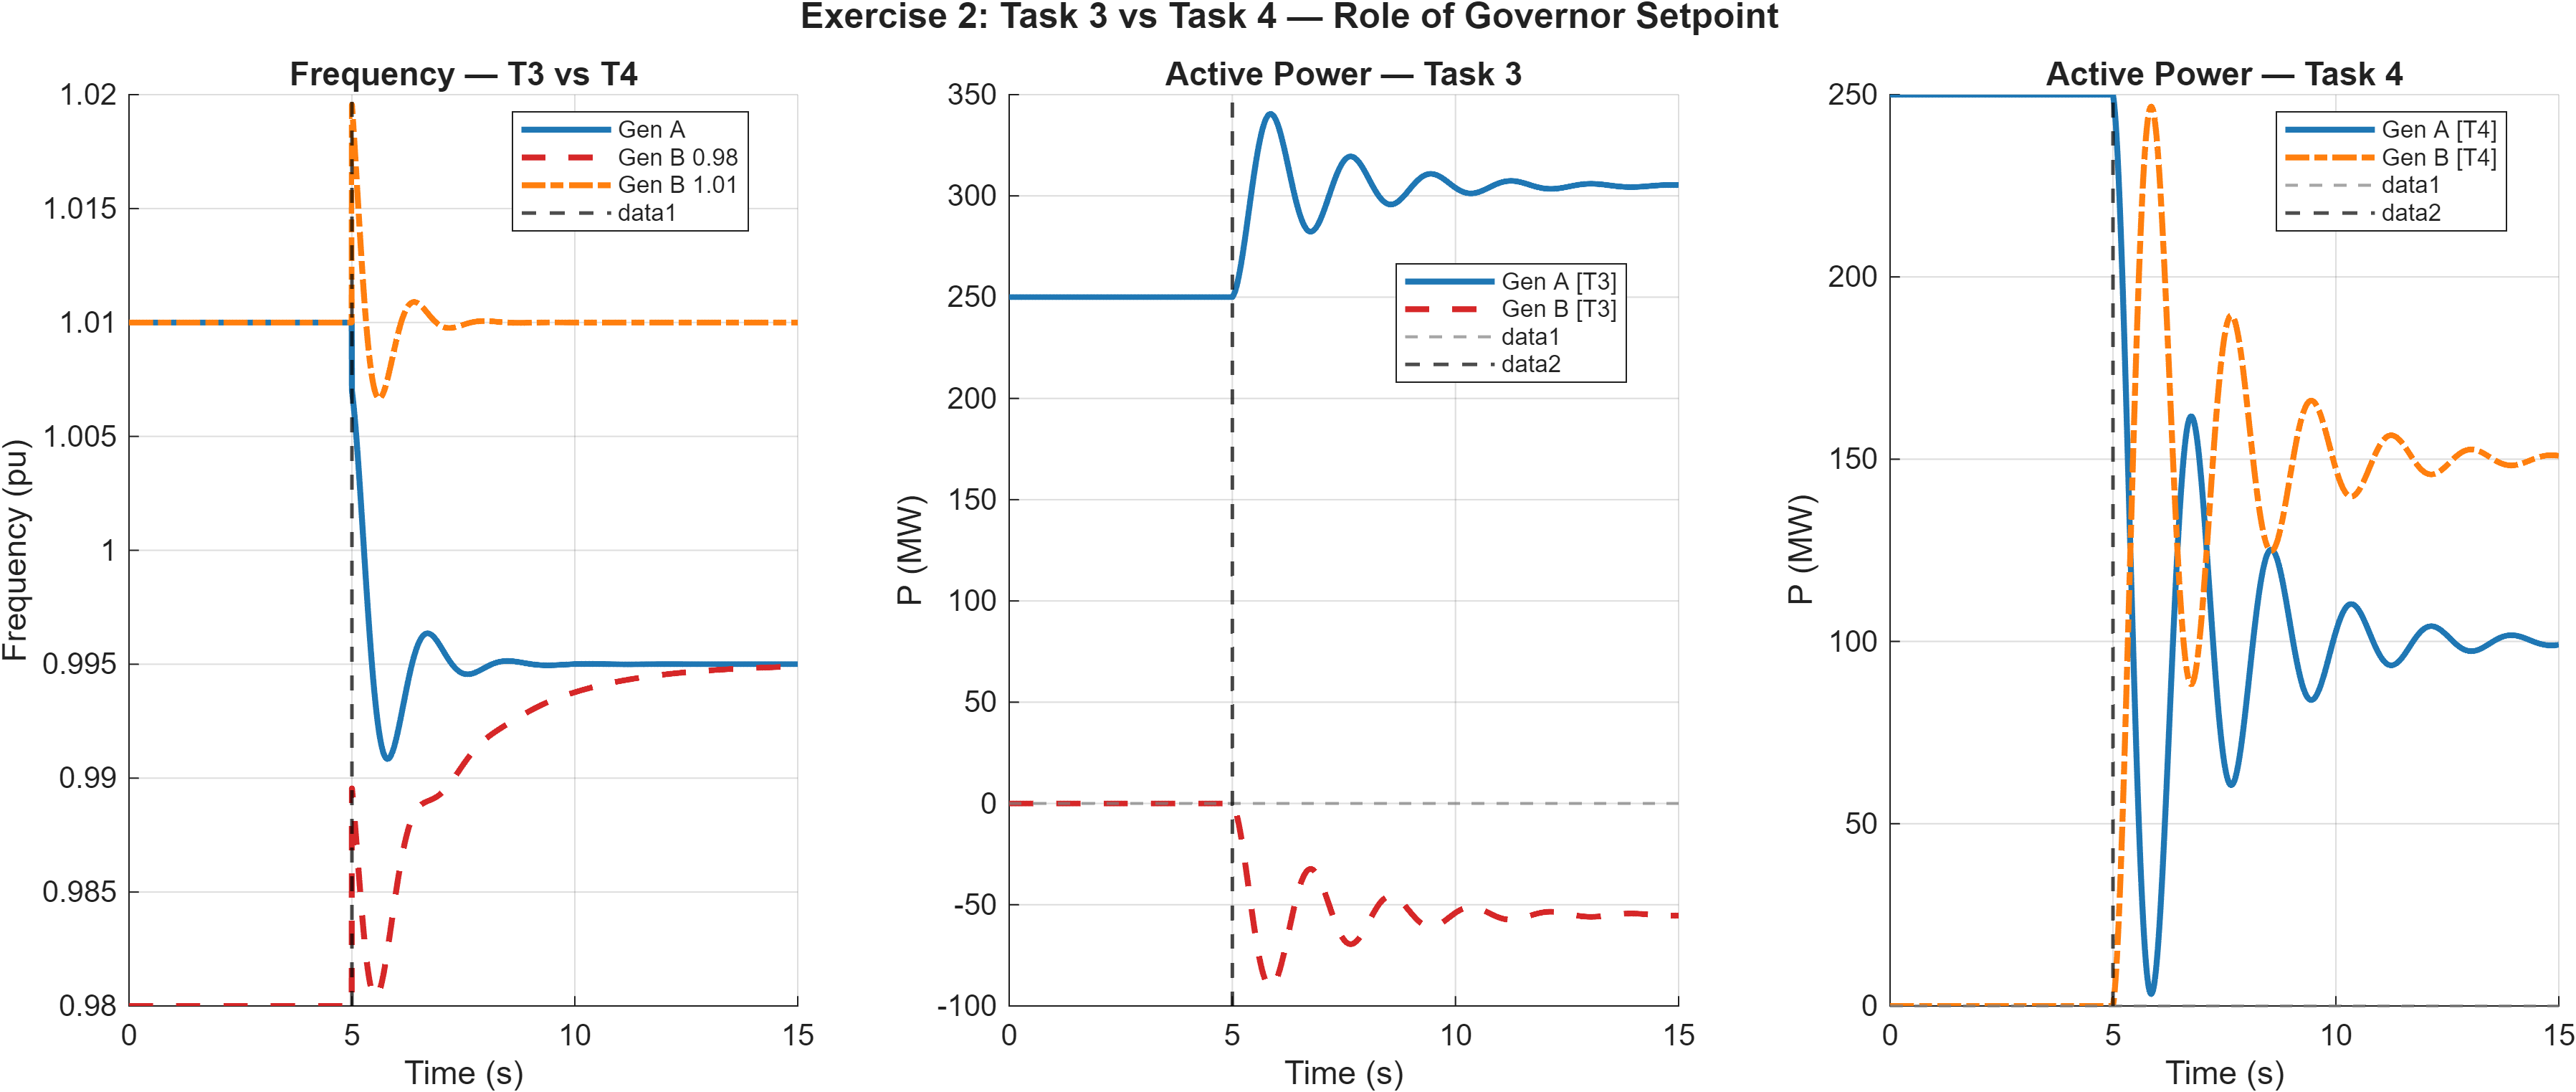
\includegraphics[width=\textwidth]{figures/Task3_vs_Task4.png}
  \caption{Direct comparison of Task~3 ($f_{\text{set},B} = \pu{0.98}$) and
    Task~4 ($f_{\text{set},B} = \pu{1.01}$). The governor setpoint alone
    determines whether Gen~B motors (Task~3) or generates (Task~4).}
  \label{fig:task3_vs_task4}
\end{figure}

The comparison confirms the core principle: the governor frequency setpoint is
the \emph{sole} determinant of active power sharing in parallel operation. An
under-frequency oncoming machine (Task~3) absorbs power --- a hazardous motoring
condition, while an over-frequency machine (Task~4) assumes the majority of the
system load.
